\begin{figure*}[t]
    \centering
    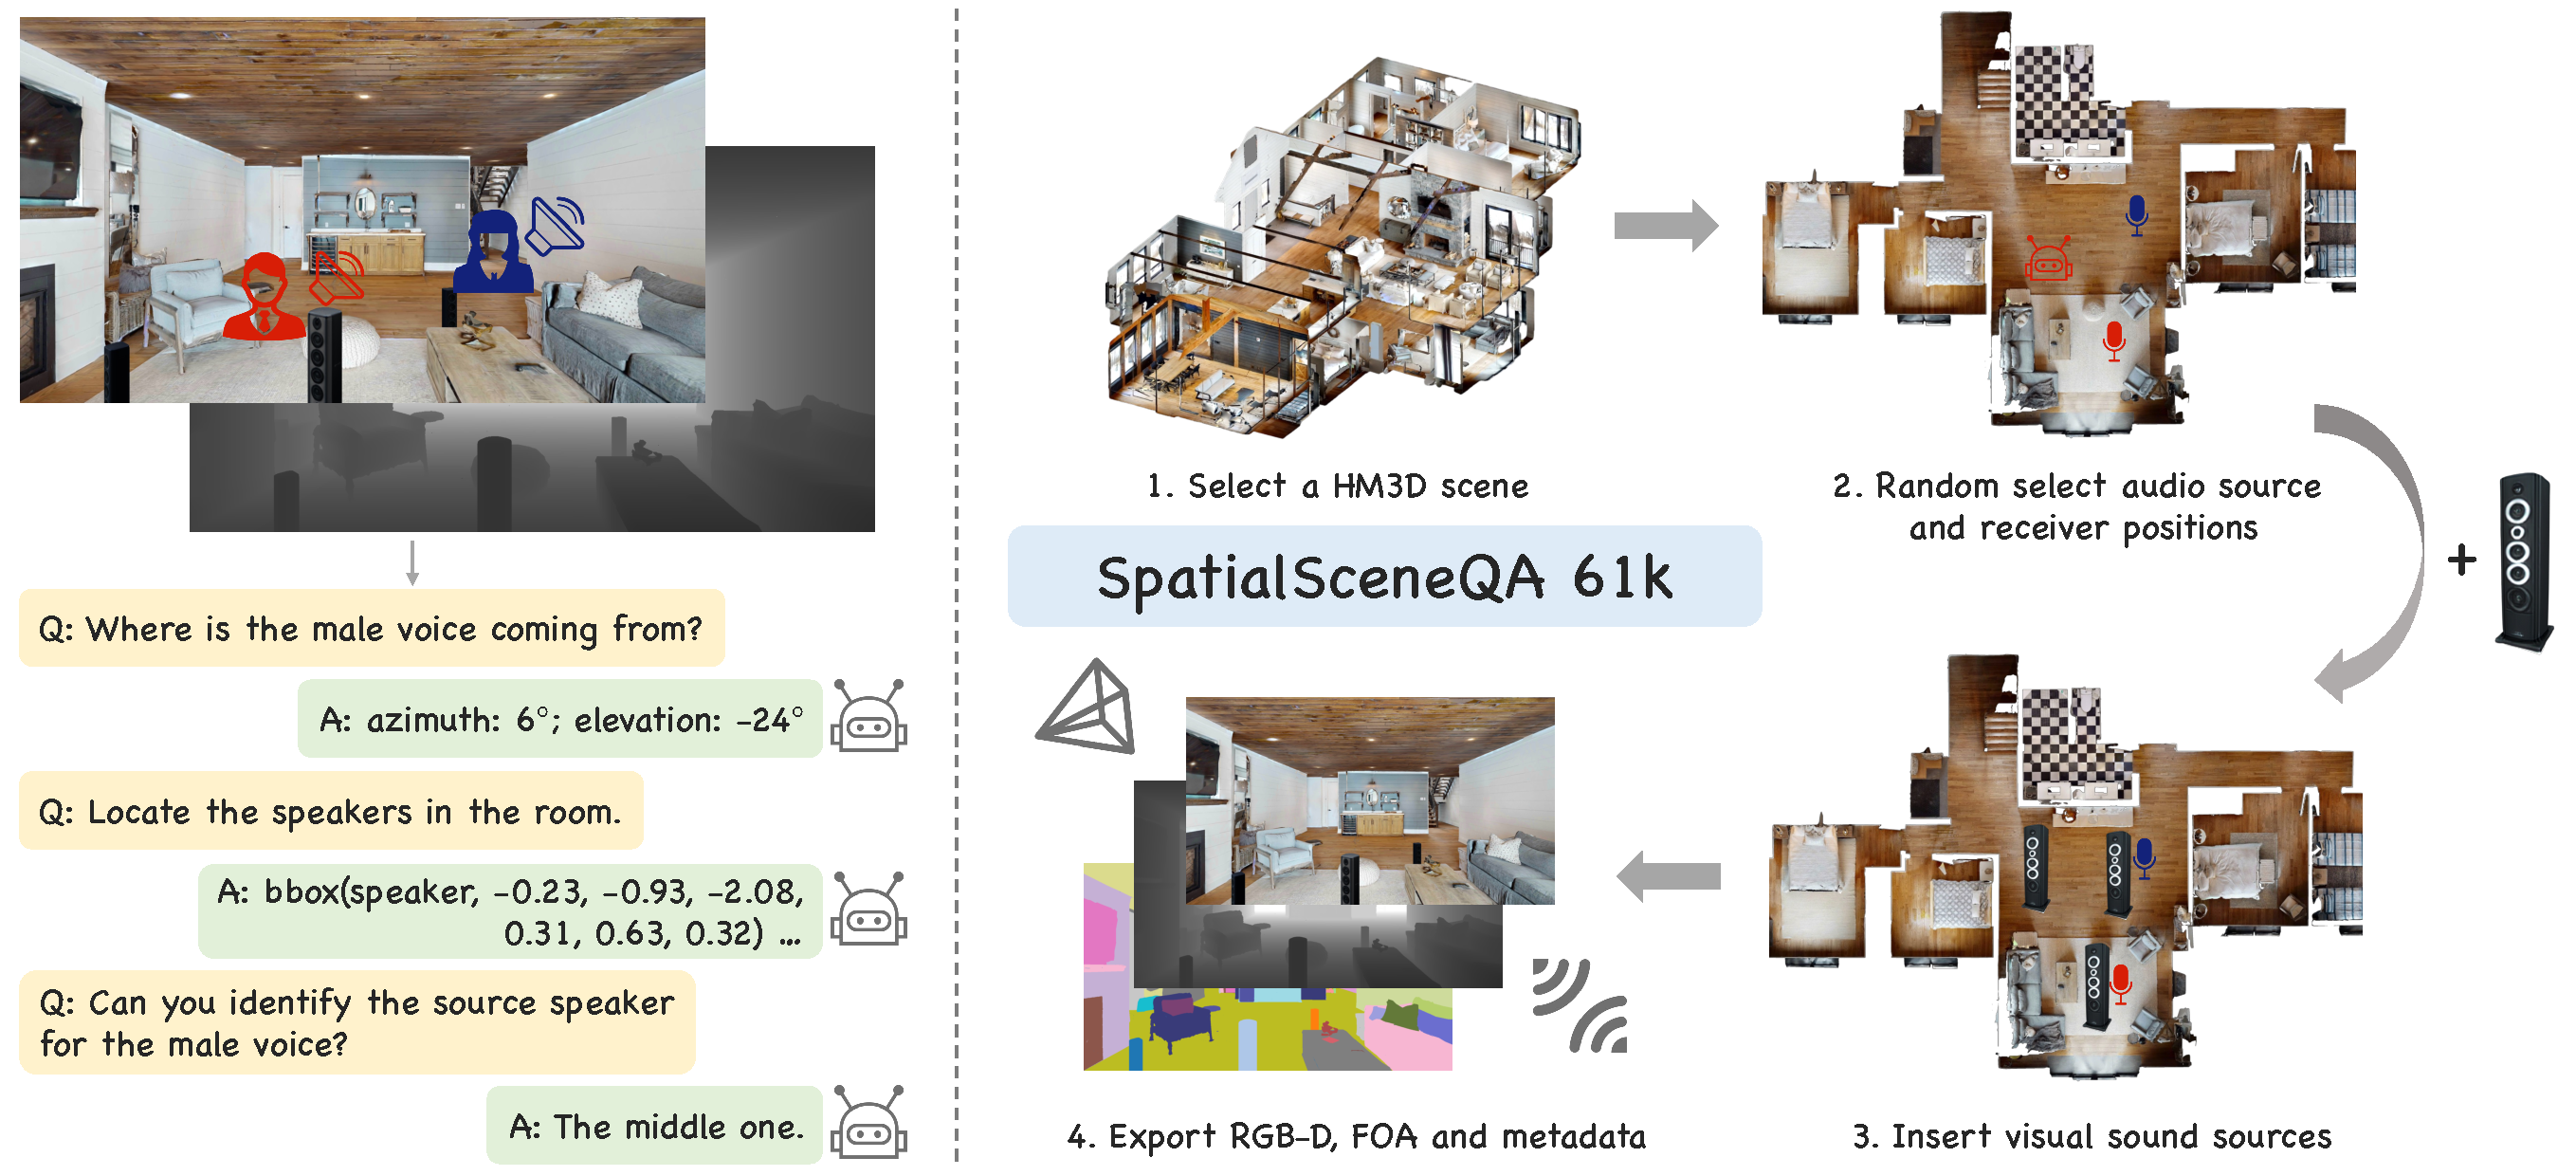
\includegraphics[width=1.0\linewidth]{data-pipeline-2.pdf}
\caption{\textbf{Overview of the \textsc{SpatialSceneQA} 61k dataset.}. \textbf{Left:} Example question-answer pairs demonstrating diverse spatial tasks, including sound source localization (azimuth/elevation), visual grounding (bounding boxes), and overlapping sound source identification. \textbf{Right:} The data synthesis pipeline leveraging \textit{Habitat-Sim} and \textit{SoundSpaces 2.0}. The process consists of four stages: (1) selecting an HM3D scene, (2) sampling random source and receiver poses, (3) inserting 3D visual sound sources (e.g., speakers generated by Hunyuan3D-1.0), and (4) exporting synchronized RGB-D frames, FOA audio, and semantic and camera intrinsic/extrinsic metadata.}   
    \label{fig:pipeline}
\end{figure*}

\section{Related Work}

\subsection{Spatial Audio Understanding}

Spatial audio understanding seeks to infer the spatial configuration of acoustic events from multi-channel recordings, including binaural signals, FOA, and microphone arrays. Early work has primarily focused on sound event localization and detection \citep{adavanne2018sound, cao2021improved, shimada2021accdoa, shimada2022multi}, where models jointly estimate event activity and coarse spatial attributes. Recent studies have begun to integrate spatial audio perception with large language models (LLMs), enabling instruction following and higher-level reasoning grounded in spatial acoustic cues.

A major design choice is the spatial representation. 
Binaural modeling leverages interaural time and level differences and head-related transfer functions (HRTFs) induced cues, and recent geometry-aware encoders improve the use of such signals \citep{zheng2024bat, biswas2025owl}. 
However, binaural cues are tightly coupled to recording geometry and the underlying HRTFs, which hinders generalization across devices. 
FOA has a hardware-agnostic alternative by encoding spatial information in the B-format. 
\citep{devnani2024learning} aligns FOA-based spatial embeddings with semantics via contrastive learning, while \citep{tang2024can} injects intensity vector cues into an auditory LLM to support localization and localization-conditioned speech processing.

Progress in this area is further constrained by data availability. 
Real-world multi-channel datasets with dense spatial annotations remain scarce, with STARSS23 \citep{shimada2023starss23} serving as a representative benchmark. 
However, STARSS23 pairs multi-channel audio with RGB-only paranomic video, and does not provide depth aligned to the visual stream. 
This limitation has motivated simulation-driven data generation, where configurable simulators such as SoundSpaces 2.0 \citep{chen22soundspaces2} enable scalable synthesis of reverberant or anechoic audio-visual data with controllable scene geometry and precise ground-truth spatial annotations.

\subsection{Visual 3D Object Grounding}

Three-dimensional visual grounding and spatial reasoning have become increasingly important for modern vision–language models \citep{huang2024chat, chen2024grounded, Qwen3-VL, guo2025seed1, zhu2025internvl3} and AV-LLMs \citep{senocak2023sound, chowdhury2024meerkat, li2024groundinggpt}, as many downstream tasks demand object-level localization and relational reasoning beyond two-dimensional captioning. Existing approaches primarily differ along two dimensions: (i) how 3D geometric information is incorporated and (ii) whether the model natively predicts 3D outputs.

A first line of work conditions models on explicit 3D structure, such as point clouds or object-centric 3D tokens, to impose direct geometric constraints \citep{huang2024chat, mao2025spatiallm}. 
An alternative relies on multi-view video or RGB-D streams as implicit 3D supervision \citep{qi2025gpt4scene, zheng2025video, chen2024spatialvlm, zhu2024llava}. 
\citep{zheng2025video} projects depth into global coordinates and injects 3D positional encodings into video representations, improving spatial awareness through geometry-aligned tokens. 
Similarly, RGB-D-based approaches incorporate depth-derived cues into visual tokens to strengthen geometric grounding \citep{chen2024spatialvlm, zhu2024llava}.

Several approaches rely on auxiliary components to obtain reliable 3D signals, such as external 3D segmenters for candidate proposal generation or specialized decoders for 3D grounding \citep{zheng2025video, zhu2024llava}. More recently, N3D-VLM \citep{wang2025n3d} advances a more native paradigm by explicitly reasoning about and directly predicting 3D bounding boxes within the model.

\subsection{AV-LLMs for 3D Understanding}

Recent AV-LLMs show strong multimodal understanding \citep{cheng2024videollama, xu2025qwen2, Qwen3-Omni, tang2025video}, but are largely trained on RGB video and monaural audio, leaving spatial structure and directional acoustics implicit. This limitation motivates a line of work that augments AV-LLMs with explicit spatial cues for precise localization and geometric reasoning. One representative approach builds modular pipelines that estimate geometry and spatial acoustics using specialized components, while delegating higher-level reasoning to an LLM. \citep{chen2025savvy} introduces a benchmark for dynamic 3D audio-visual spatial reasoning with synchronized spatial audio and proposes a training-free pipeline that estimates object trajectories and constructs a global spatial map to answer queries. Complementary simulation-based efforts, such as Hear You Are \citep{ryu2025hear}, exploit panoramic imagery and binaural audio cues for audio-visual spatial reasoning, but continue to rely on RGB-only visual inputs, leaving explicit depth information unmodeled.

In contrast, our work adapts an existing AV-LLM to directly perceive and reason about spatial cues by incorporating RGB-D observations and FOA-based multi-channel audio in an end-to-end manner. We introduce a learned spatial audio representation, the Neural IV, and construct a large-scale instruction-tuning dataset, SpatialSceneQA, to jointly support spatial perception, grounding, and language-based reasoning within a unified framework.
